\documentclass[tikz,border=8pt]{standalone}
\usetikzlibrary{calc,arrows.meta}

\begin{document}
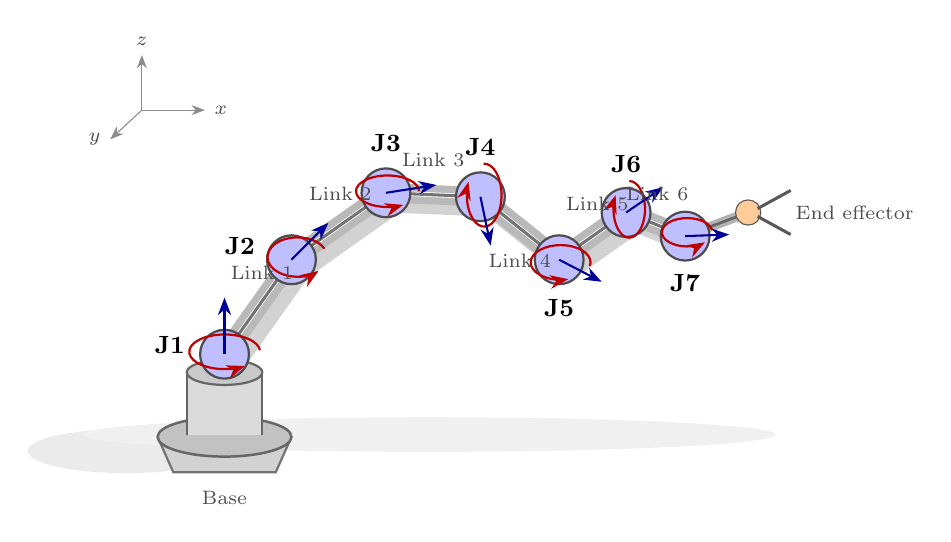
\begin{tikzpicture}[
  x=1cm,y=1cm,
  >=Stealth,
  joint/.style={circle, draw=black!70, fill=blue!25, line width=0.8pt, minimum size=0.62cm},
  link/.style={line width=7pt, line cap=round, draw=gray!55},
  linkedge/.style={line width=1.1pt, line cap=round, draw=black!55},
  axisarrow/.style={->, line width=0.8pt, draw=red!75!black},
  label/.style={font=\small\bfseries, text=black},
  note/.style={font=\scriptsize, text=black!70}
]

% Coordinates for a slightly 3D-looking 7-axis robot arm
\coordinate (B0) at (0,0);
\coordinate (J1) at (0,1.05);
\coordinate (J2) at (0.85,2.25);
\coordinate (J3) at (2.05,3.10);
\coordinate (J4) at (3.25,3.05);
\coordinate (J5) at (4.25,2.25);
\coordinate (J6) at (5.10,2.85);
\coordinate (J7) at (5.85,2.55);
\coordinate (TCP) at (6.65,2.85);

% Soft ground shadow
\fill[black!8] (-1.25,-0.18) ellipse (1.25 and 0.28);
\fill[black!6] (2.6,0.03) ellipse (4.4 and 0.22);

% Base, drawn as simple pseudo-3D cylinders
\fill[gray!35] (-0.85,0) -- (-0.65,-0.45) -- (0.65,-0.45) -- (0.85,0) -- cycle;
\draw[black!55, line width=0.8pt] (-0.85,0) -- (-0.65,-0.45) -- (0.65,-0.45) -- (0.85,0);
\fill[gray!48] (0,0) ellipse (0.85 and 0.25);
\draw[black!60, line width=0.9pt] (0,0) ellipse (0.85 and 0.25);
\fill[gray!28] (-0.48,0.02) rectangle (0.48,0.82);
\fill[gray!42] (0,0.82) ellipse (0.48 and 0.16);
\draw[black!60, line width=0.8pt] (-0.48,0.02) -- (-0.48,0.82);
\draw[black!60, line width=0.8pt] (0.48,0.02) -- (0.48,0.82);
\draw[black!60, line width=0.8pt] (0,0.82) ellipse (0.48 and 0.16);
\node[note] at (0,-0.78) {Base};

% Link shadows/offsets for depth
\draw[link, draw=gray!35] ($(J1)+(0.13,-0.13)$) -- ($(J2)+(0.13,-0.13)$);
\draw[link, draw=gray!35] ($(J2)+(0.13,-0.13)$) -- ($(J3)+(0.13,-0.13)$);
\draw[link, draw=gray!35] ($(J3)+(0.13,-0.13)$) -- ($(J4)+(0.13,-0.13)$);
\draw[link, draw=gray!35] ($(J4)+(0.13,-0.13)$) -- ($(J5)+(0.13,-0.13)$);
\draw[link, draw=gray!35] ($(J5)+(0.13,-0.13)$) -- ($(J6)+(0.13,-0.13)$);
\draw[link, draw=gray!35] ($(J6)+(0.13,-0.13)$) -- ($(J7)+(0.13,-0.13)$);

% Main links
\draw[link] (J1) -- (J2);
\draw[link] (J2) -- (J3);
\draw[link] (J3) -- (J4);
\draw[link] (J4) -- (J5);
\draw[link] (J5) -- (J6);
\draw[link] (J6) -- (J7);

% Link highlights and edges
\draw[linkedge, draw=white!80, line width=1.7pt] (J1) -- (J2);
\draw[linkedge, draw=white!80, line width=1.7pt] (J2) -- (J3);
\draw[linkedge, draw=white!80, line width=1.7pt] (J3) -- (J4);
\draw[linkedge, draw=white!80, line width=1.7pt] (J4) -- (J5);
\draw[linkedge, draw=white!80, line width=1.7pt] (J5) -- (J6);
\draw[linkedge, draw=white!80, line width=1.7pt] (J6) -- (J7);
\draw[linkedge] (J1) -- (J2);
\draw[linkedge] (J2) -- (J3);
\draw[linkedge] (J3) -- (J4);
\draw[linkedge] (J4) -- (J5);
\draw[linkedge] (J5) -- (J6);
\draw[linkedge] (J6) -- (J7);

% End effector
\draw[line width=3.5pt, line cap=round, draw=gray!60] (J7) -- (TCP);
\draw[line width=1pt, draw=black!60] (J7) -- (TCP);
\fill[orange!40] (TCP) circle (0.16);
\draw[black!65] (TCP) circle (0.16);
\draw[line width=1.1pt, draw=black!65] ($(TCP)+(0.12,0.05)$) -- ++(0.42,0.23);
\draw[line width=1.1pt, draw=black!65] ($(TCP)+(0.12,-0.05)$) -- ++(0.42,-0.23);
\node[note, anchor=west] at ($(TCP)+(0.48,0)$) {End effector};

% Joints
\node[joint] at (J1) {};
\node[joint] at (J2) {};
\node[joint] at (J3) {};
\node[joint] at (J4) {};
\node[joint] at (J5) {};
\node[joint] at (J6) {};
\node[joint] at (J7) {};

% Joint labels
\node[label, anchor=east] at ($(J1)+(-0.38,0.12)$) {J1};
\node[label, anchor=east] at ($(J2)+(-0.34,0.18)$) {J2};
\node[label, anchor=south] at ($(J3)+(0,0.40)$) {J3};
\node[label, anchor=south] at ($(J4)+(0,0.40)$) {J4};
\node[label, anchor=north] at ($(J5)+(0,-0.38)$) {J5};
\node[label, anchor=south] at ($(J6)+(0,0.38)$) {J6};
\node[label, anchor=north] at ($(J7)+(0,-0.36)$) {J7};

% Rotation direction arrows for each axis
\draw[axisarrow] ($(J1)+(0.45,0.05)$) arc[start angle=5,end angle=305,x radius=0.45,y radius=0.22];
\draw[axisarrow] ($(J2)+(0.42,0.14)$) arc[start angle=25,end angle=315,x radius=0.38,y radius=0.25];
\draw[axisarrow] ($(J3)+(0.42,0.02)$) arc[start angle=0,end angle=300,x radius=0.40,y radius=0.20];
\draw[axisarrow] ($(J4)+(0.04,0.42)$) arc[start angle=92,end angle=-205,x radius=0.22,y radius=0.40];
\draw[axisarrow] ($(J5)+(0.39,-0.08)$) arc[start angle=-12,end angle=285,x radius=0.38,y radius=0.22];
\draw[axisarrow] ($(J6)+(0.04,0.40)$) arc[start angle=90,end angle=-210,x radius=0.20,y radius=0.36];
\draw[axisarrow] ($(J7)+(0.34,0.08)$) arc[start angle=10,end angle=315,x radius=0.32,y radius=0.18];

% Axis hints
\draw[->, line width=0.75pt, draw=blue!60!black] (J1) -- ++(0,0.72);
\draw[->, line width=0.75pt, draw=blue!60!black] (J2) -- ++(0.47,0.47);
\draw[->, line width=0.75pt, draw=blue!60!black] (J3) -- ++(0.64,0.10);
\draw[->, line width=0.75pt, draw=blue!60!black] (J4) -- ++(0.13,-0.62);
\draw[->, line width=0.75pt, draw=blue!60!black] (J5) -- ++(0.54,-0.28);
\draw[->, line width=0.75pt, draw=blue!60!black] (J6) -- ++(0.47,0.32);
\draw[->, line width=0.75pt, draw=blue!60!black] (J7) -- ++(0.56,0.02);

% Relationship captions
\node[note, anchor=south] at ($(J1)!0.5!(J2)+(0.05,0.22)$) {Link 1};
\node[note, anchor=south] at ($(J2)!0.5!(J3)+(0.02,0.20)$) {Link 2};
\node[note, anchor=south] at ($(J3)!0.5!(J4)+(0,0.23)$) {Link 3};
\node[note, anchor=north] at ($(J4)!0.5!(J5)+(0,-0.20)$) {Link 4};
\node[note, anchor=south] at ($(J5)!0.5!(J6)+(0.06,0.20)$) {Link 5};
\node[note, anchor=south] at ($(J6)!0.5!(J7)+(0.02,0.18)$) {Link 6};

% Small depth cue axes
\draw[->, thin, draw=black!45] (-1.05,4.15) -- (-0.25,4.15) node[right, note] {$x$};
\draw[->, thin, draw=black!45] (-1.05,4.15) -- (-1.05,4.85) node[above, note] {$z$};
\draw[->, thin, draw=black!45] (-1.05,4.15) -- (-1.45,3.78) node[left, note] {$y$};

\end{tikzpicture}
\end{document}
